\chapter{Canonical Quantization}

    The main reference for this chapter is \cite{Peskin}.

    ?? CHECK THIS CHAPTER AND FIX IT ??

\section{Klein-Gordon field}\index{Klein-Gordon equation}
\subsection{Lagrangian and Hamiltonian}

    The ``simplest'' Lagrangian (density) is given by
    \begin{gather}
        \label{qft:klein_gordon_lagrangian}
        \mathcal{L} = \frac{1}{2}\partial_\mu\phi\partial^\mu\phi - \frac{1}{2}m^2\phi^2.
    \end{gather}
    Using the principle of least action, the following Euler-Lagrange equation is obtained:
    \begin{gather}
        \left(\partial^\mu\partial_\mu + m^2\right)\phi = 0.
    \end{gather}
    This can be rewritten using the \textbf{d'Alembertian} $\Box = \partial_\mu\partial^\mu$:\index{d'Alembert!operator}\nomenclature[O_dAl]{$\Box$}{d'Alembert operator}
    \begin{gather}
        \label{qft:klein_gordon_equation}
        (\Box+m^2)\phi = 0.
    \end{gather}
    This equation is called the \textbf{Klein-Gordon equation}. In the limit $m\rightarrow0$ this equation reduces to the well-known wave equation.

    From the Lagrangian \eqref{qft:klein_gordon_lagrangian} one can also derive a Hamiltonian function using relations \ref{lagrange:conjugate_momentum} and \ref{lagrange:hamiltonian}:
    \begin{gather}
        \label{qft:klein_gordon_hamiltonian}
        H = \frac{1}{2}\int d^3x\left[\pi^2(x) + (\nabla\phi(x))^2 + m^2\phi^2(x)\right].
    \end{gather}

\subsection{Raising and lowering operators}

    Fourier transforming the scalar field $\phi(\vector{x},t)$ in momentum space and inserting it into the Klein-Gordon equation gives
    \begin{gather}
        \left(\partial_t^2+p^2+m^2\right)\phi(\vector{p},t) = 0.
    \end{gather}
    This is the equation for a simple harmonic oscillator with frequency $\omega = \sqrt{p^2 + m^2}$.

    Analogous to ordinary quantum mechanics, raising and lowering operators $a_{\vector{p}}^\dag$ and $a_{\vector{p}}$ can be defined such that
    \begin{align}
        \phi(\vector{x}) &= \iiint\frac{d^3p}{(2\pi)^{3/2}}\frac{1}{\sqrt{2\omega_{\vector{p}}}}\left(a_{\vector{p}}e^{i\vector{p}\cdot\vector{x}} + a_{\vector{p}}^\dag e^{-i\vector{p}\cdot\vector{x}}\right)\label{qft:phi}\\
        \pi(\vector{x}) &= \iiint\frac{d^3p}{(2\pi)^{3/2}}(-i)\sqrt{\frac{\omega_{\vector{p}}}{2}}\left(a_{\vector{p}}e^{i\vector{p}\cdot\vector{x}} - a_{\vector{p}}^\dag e^{-i\vector{p}\cdot\vector{x}}\right).
    \end{align}
    An equivalent definition is obtained by performing the transformation $\vector{p}\longrightarrow-\vector{p}$ in the second term of $\phi(\vector{x})$ and $\pi(\vector{x})$:
    \begin{align}
        \phi(\vector{x}) &= \iiint\frac{d^3p}{(2\pi)^{3/2}}\frac{1}{\sqrt{2\omega_{\vector{p}}}}\left(a_{\vector{p}} + a_{-\vector{p}}^\dag\right)e^{i\vector{p}\cdot\vector{x}}\\
        \pi(\vector{x}) &= \iiint\frac{d^3p}{(2\pi)^{3/2}}(-i)\sqrt{\frac{\omega_{\vector{p}}}{2}}\left(a_{\vector{p}} - a_{-\vector{p}}^\dag\right)e^{i\vector{p}\cdot\vector{x}}.
    \end{align}

    When the commutation relation
    \begin{gather}
        \label{qft:ladder_comutation}
        [a_{\vector{p}},a_{\vector{q}}^\dag] := \delta(\vector{p}-\vector{q})
    \end{gather}
    is imposed, the following commutation relation for the scalar field and its conjugate momentum is obtained:
    \begin{gather}
        [\phi(\vector{x}),\pi(\vector{y})] = i\delta(\vector{x} - \vector{y}).
    \end{gather}
    Now, the Hamiltonian can be calculated explicitly:
    \begin{gather}
        \label{qft:Klein_gordon_hamiltonian}
        H = \int\frac{d^3p}{(2\pi)^3}\omega_{\vector{p}}\left(a_{\vector{p}}^\dag a_{\vector{p}} + \frac{1}{2}[a_{\vector{p}}, a_{\vector{p}}^\dag]\right).
    \end{gather}
    However, it is clear from Equation \eqref{qft:ladder_comutation} that the second term in this integral diverges. There are two reasons for this divergence. First, space is infinite, i.e. the $d^3x$ integral in \eqref{qft:klein_gordon_hamiltonian} diverges. This problem can be resolved by restricting the system to a (finite) part of space or by considering the energy density instead of the energy itself. Second, by including very large values for $p$ in the integral, a parameter range is explored where the theory is likely to break down. To resolve this problem a  ``high $p$''-cut-off should be introduced. A more practical solution, however, is to note that only energy differences are physical and so one can simply drop the second term altogether as it is merely a ``constant'' (albeit an infinite one).

    A corollary of Equation \eqref{qft:Klein_gordon_hamiltonian} together with the canonical commutation relations is
    \begin{align}
        [H,a_{\vector{p}}^\dag] &= \omega_pa_{\vector{p}}^\dag\\
        [H,a_{\vector{p}}] &= -\omega_pa_{\vector{p}}.
    \end{align}
    As was the case for the quantum harmonic oscillator, the creation and annihilation operators deserve their names and one can write:
    \begin{gather}
        |\vector{k}_1,\ldots,\vector{k}_n\rangle = a^\dag(\vector{k}_1)\cdots a^\dag(\vector{k}_n)|0\rangle.
    \end{gather}
    Furthermore, this equation together with the canonical commutation relations imply that the Klein-Gordon fields are bosonic fields.

\subsection{Scalar propagator}

    \newformula{Pauli-Jordan function}{\index{Pauli-Jordan function}
        \begin{gather}
            i\Delta(x-y) := i[\phi(x), \phi(y)] = \int\frac{d^3p}{(2\pi)^3}\frac{1}{2\omega_p}\left(e^{-i\mathbf{p}\cdot(\mathbf{x}-\mathbf{y})} - e^{i\mathbf{p}\cdot(\mathbf{x}-\mathbf{y})}\right)
        \end{gather}
        In the case that $x^0 = y^0$ (ETCR) or $(x-y)^2 < 0$ (spacelike curves), the Pauli-Jordan function is identically 0. (See also the \textit{axiom of microcausality} \ref{aqft:microcausality}).
    }

\subsection{Normalization constant}

    By Property \ref{distribution:delta_of_function} the delta function $\delta^{(3)}(\vector{p}-\vector{q})$ transforms as $\delta^{(3)}(\Lambda\vector{p} - \Lambda\vector{q})\frac{\Lambda E}{E}$ under a general Lorentz boost $\Lambda$. Although this is clearly not Lorentz invariant, the quantity $E_p\delta^{(3)}(\vector{p}-\vector{q})$ can be seen to be invariant.

    The correct normalization for the momentum representation becomes
    \begin{gather}
        \sqrt{2E_p}a_{\mathbf{p}}^\dag|0\rangle = |\mathbf{p}\rangle
    \end{gather}
    and, hence,
    \begin{gather}
        \langle\mathbf{p}|\mathbf{q}\rangle = 2E_p(2\pi)^3\delta^{(3)}(\vector{p}-\vector{q}),
    \end{gather}
    where the constants are a matter of convention to cancel the constants in expression \eqref{qft:phi}.

\subsection{Invariant integration measure}

    The factor $2E_p$ does not only occur in the normalization conditions. To find a Lorentz invariant integration measure in spacetime, the following integral can be studied:
    \begin{gather}
        \int\frac{d^3p}{2E_p} = \left.\int\delta(p^2-m^2)d^4p\,\right|_{p^0>0}.
    \end{gather}
    By using this measure it is ensured that the integral of any Lorentz invariant function is again Lorentz invariant.
    \begin{example}[One-particle identity operator]\index{identity!operator}
        \begin{gather}
            \mathbbm{1} := \int\frac{d^3p}{2E_p}|\mathbf{p}\rangle\langle\mathbf{p}|
        \end{gather}
    \end{example}

\section{Contractions and Wick's theorem}
\subsection{Bosonic fields}

    In the following definitions (field) operators will be decomposed as \[\phi = \phi^{(+)} + \phi^{(-)},\] where the + symbol denotes the ``positive frequency'' part, i.e. the part consisting of annihilation operators. The ``negative frequency'' part is defined analogously. This terminology stems from the classic Fourier integral. By looking at Equation \eqref{qft:phi} and remembering that the $(1,3)$-signature is adopted,the annihilators can be seen to always occur together with a positive frequency exponential.

    \newdef{Contraction for neutral bosonic fields}{\index{contraction}
        \begin{gather}
            \contraction{}{\phi}{(x)}{\phi}\phi(x)\phi(y) :=
            \begin{cases}
                [\phi(x)^{(+)},\phi(y)^{(-)}]&x^0>y^0\\
                [\phi(y)^{(+)},\phi(x)^{(-)}]&y^0>x^0
            \end{cases}
        \end{gather}
    }
    \newformula{Feynman propagator}{\index{Feynman!propagator}
        \begin{gather}
            i\Delta_F(x-y) := \contraction{}{\phi}{(x)}{\phi}\phi(x)\phi(y) := i\lim_{\varepsilon\rightarrow 0^+}\int\frac{d^4p}{(2\pi)^4}\frac{e^{-ip\cdot(x-y)}}{p^2 - m^2 + i\varepsilon}
        \end{gather}
    }

    \newdef{Contraction for charged bosonic fields}{
        \begin{gather}
            \contraction{}{\phi}{(x)}{\overline\phi}\phi(x)\overline\phi(y) :=
            \begin{cases}
                [\phi(x)^{(+)},\overline\phi(y)^{(-)}]&x^0>y^0\\
                [\phi(y)^{(+)},\overline\phi(x)^{(-)}]&y^0>x^0
            \end{cases}
        \end{gather}
    }

    \newdef{Normal ordering}{\index{normal!ordering}
        The normal ordering $\mathcal{N}$ (also often denoted by colons $:\ \ :$) of a sequence of field operators is defined as the permuted sequence in which all annihilation operators appear on the right of the creation operators, e.g.: \[\mathcal{N}\Big(\phi(x)\phi^\dag(y)\phi(z)\Big) = \phi^\dag(y)\phi(x)\phi(z).\] In fact the normal ordering operator is not a morphism between CCR-algebras since this would lead to a contradiction: \[b_ib_j^\dag = b_j^\dag b_i + \delta_{ij}\implies\mathcal{N}(b_ib_j^\dag) = \mathcal{N}(b_j^\dag b_i+\delta_{ij}) = \mathcal{N}(b_j^\dag b_i) + \delta_{ij}\implies\delta_{ij}\equiv0.\] The solution is given by the fact that inside the normal ordering all operators commute and, hence, this ordering can be axiomatized as an algebra morphism $\mathcal{N}:\Sym^\bullet A\rightarrow A$ where $A$ is the CCR-algebra of the theory (see \cite{miwa}).
    }
    \begin{property}
        From this definition it immediately follows that the vacuum expectation value of a normal ordered sequence is 0.
    \end{property}

    \newformula{Wick's theorem for bosonic fields}{\index{Wick!theorem for time-ordered integrals}
        \begin{gather}
            \mathcal{T}\Big(\phi(x_1)\phi(x_2)\cdots\phi(x_n)\Big) = \mathcal{N}\Big(\phi(x_1)\cdots\phi(x_n) + \text{all possible contractions}\Big)
        \end{gather}
    }

    \begin{remark}
        In the case of charged bosons, only contractions of the form $\contraction{}{\phi}{(x)}{\overline\phi}\phi(x)\overline\phi(y)$ will remain because $[a,b^+] = 0$.
    \end{remark}

\subsection{Fermionic fields}

    \newdef{Contraction}{
        \begin{gather}
            \contraction{}{\psi}{(x)}{\overline\psi}\psi(x)\overline\psi(y) :=
            \begin{cases}
                \{\psi(x)^{(+)},\overline\psi(y)^{(-)}\}_+&x^0>y^0\\
                -\{\psi(y)^{(+)},\overline\psi(x)^{(-)}\}_+&y^0>x^0
            \end{cases}
        \end{gather}
    }
    \begin{remark}
        Only contractions of the form $\contraction{}{\psi}{(x)}{\overline\psi}\psi(x)\overline\psi(y)$ will remain because $\{a,b^\dag\}_+ = 0$.
    \end{remark}

    \newformula{Feynman propagator}{\index{Feynman!propagator}
        \begin{gather}
            iS_F(x-y) := \contraction{}{\psi}{(x)}{\overline\psi}\psi(x)\overline\psi(y) := i\lim_{\varepsilon\rightarrow 0^+}\int\frac{d^4p}{(2\pi)^4}\frac{\slashed{p} + m}{p^2 - m^2 + i\varepsilon}e^{-ip\cdot(x-y)}
        \end{gather}
    }

    \begin{remark}[Normal ordering]
        One should take into account the Fermi-Dirac statistics when permuting fermionic field operators under a normal ordering. A general factor $\sgn(\sigma)$, where $\sigma$ is the permutation of the operators, will arise in every term, e.g.: \[\mathcal{N}\Big(\psi(x)\overline\psi(y)\psi(z)\Big) = -\overline\psi(y)\psi(x)\psi(z)\] A similar remark should be made for the time-ordering operator $\mathcal{T}$. As was the case for bosonic theories one should pay attention to the nature of the normal ordering. It is not a morphism between CAR-algebras, but instead it is an algebra morphism between a free (odd) algebra and a CAR-algebra.
    \end{remark}

\section{Feynman rules}
\subsection{Scalar theory}

    By expanding the correlation functions in perturbation theory and applying Wick's theorem, one can rewrite every term using the following dictionary for Feynman diagrams (for these rules it is assumed that every coupling constant in the Lagrangian is divided by the necessary permutation factors, e.g. in $\phi^4$-theory it is assumed that the constant is of the form $\lambda/4!$):
    \begin{itemize}
        \item Propagator $\Delta_F(x-y)$:
            \begin{gather*}
                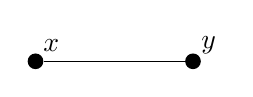
\begin{tikzpicture}
                    \node (labx) at (0.2,0.2) {$x$};
                    \node (laby) at (2.2,0.2) {$y$};
                    \node (x) at (0,0) [circle,fill,inner sep=2pt] {};
                    \node (y) at (2,0) [circle,fill,inner sep=2pt] {};
                    \draw (x) -- (y);
                \end{tikzpicture}
            \end{gather*}
        \item Interaction vertex\footnote{Four legs were drawn as an example, but this can be generalized to any order of interaction term.} $-i\lambda\int d^4z$:
            \begin{gather*}
                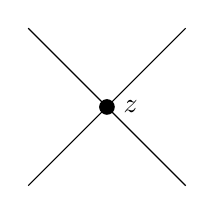
\begin{tikzpicture}
                    \node (z) at (0.3,0) {$z$};
                    \node (x) at (0,0) [circle,fill,inner sep=2pt] {};
                    \draw (-1,-1) -- (1,1);
                    \draw (-1,1) -- (1,-1);
                \end{tikzpicture}
            \end{gather*}
    \end{itemize}
    The main idea of these rules is to draw all possible diagrams consistent with the given interaction Lagrangian and translate them into analytic expressions. However, to obtain the correct normalization, one should take the following remark into account:
    \begin{remark}\index{symmetry!factor}
        Symmetry factors of diagrams should be accounted for in analytic expressions. As an example consider the following vacuum bubble:
        \begin{gather*}
            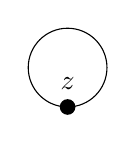
\begin{tikzpicture}
                \node (z) at (0, 0.3) {$z$};
                \node (x) at (0,0) [circle,fill,inner sep=2pt] {};
                \draw (0,0.5) circle (0.5);
            \end{tikzpicture}
        \end{gather*}
        Because the two legs can be interchanged, this diagram has \textbf{symmetry factor} 2 and, hence, it gives the analytic expression $-\frac{i\lambda}{2}\int d^4z\Delta_F(z-z)$.
    \end{remark}